\documentclass[border=4pt]{standalone}
\usepackage{amsmath,amssymb}
\usepackage{tikz,tikz-3dplot}
\usetikzlibrary{arrows.meta,calc}
\begin{document}
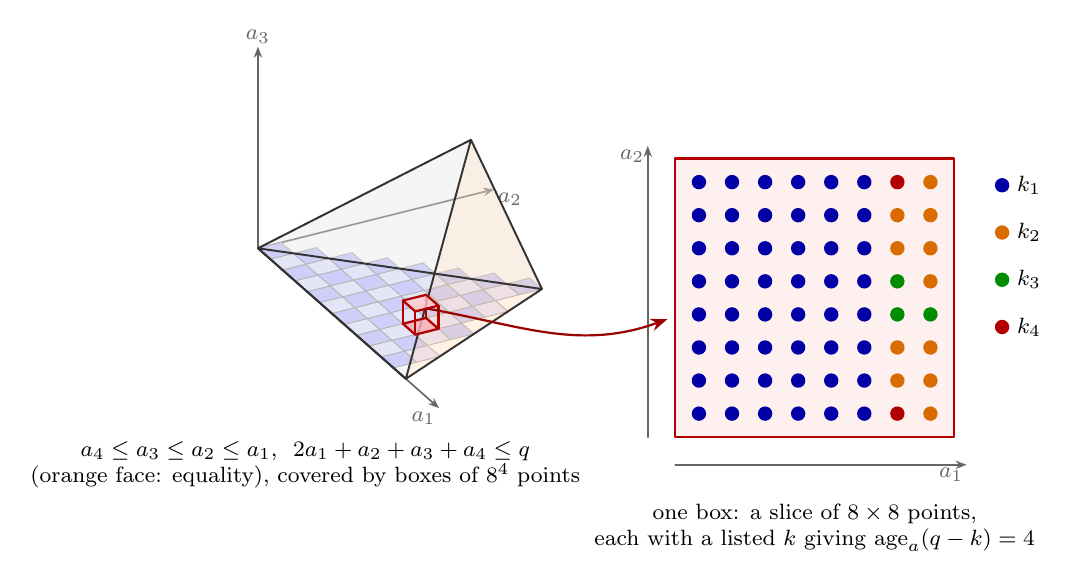
\begin{tikzpicture}[line join=round,line cap=round,
  lab/.style={font=\footnotesize,align=center,inner sep=1pt},
  axisline/.style={-{Stealth[length=4pt]},line width=0.6pt,black!60},
  arrowstep/.style={-{Stealth[length=6pt]},line width=0.8pt,gray!30!black}]
\tdplotsetmaincoords{62}{62}
\begin{scope}[tdplot_main_coords,scale=1.0]
  \coordinate (O) at (0,0,0); \coordinate (A) at (4,0,0);
  \coordinate (B) at (2.6667,2.6667,0); \coordinate (D) at (2,2,2);
  \draw[axisline] (O)--(4.9,0,0) node[lab,anchor=north east]{$a_1$};
  \draw[axisline] (O)--(0,3.4,0) node[lab,anchor=north west]{$a_2$};
  \draw[axisline] (O)--(0,0,2.9) node[lab,anchor=south]{$a_3$};
  \draw[black!35,line width=0.3pt,fill=blue!22] (0.000,0.000,0)--(0.333,0.000,0)--(0.333,0.333,0)--(0.000,0.333,0)--cycle;
  \draw[black!35,line width=0.3pt,fill=blue!10] (0.333,0.000,0)--(0.667,0.000,0)--(0.667,0.333,0)--(0.333,0.333,0)--cycle;
  \draw[black!35,line width=0.3pt,fill=blue!22] (0.333,0.333,0)--(0.667,0.333,0)--(0.667,0.667,0)--(0.333,0.667,0)--cycle;
  \draw[black!35,line width=0.3pt,fill=blue!22] (0.667,0.000,0)--(1.000,0.000,0)--(1.000,0.333,0)--(0.667,0.333,0)--cycle;
  \draw[black!35,line width=0.3pt,fill=blue!10] (0.667,0.333,0)--(1.000,0.333,0)--(1.000,0.667,0)--(0.667,0.667,0)--cycle;
  \draw[black!35,line width=0.3pt,fill=blue!22] (0.667,0.667,0)--(1.000,0.667,0)--(1.000,1.000,0)--(0.667,1.000,0)--cycle;
  \draw[black!35,line width=0.3pt,fill=blue!10] (1.000,0.000,0)--(1.333,0.000,0)--(1.333,0.333,0)--(1.000,0.333,0)--cycle;
  \draw[black!35,line width=0.3pt,fill=blue!22] (1.000,0.333,0)--(1.333,0.333,0)--(1.333,0.667,0)--(1.000,0.667,0)--cycle;
  \draw[black!35,line width=0.3pt,fill=blue!10] (1.000,0.667,0)--(1.333,0.667,0)--(1.333,1.000,0)--(1.000,1.000,0)--cycle;
  \draw[black!35,line width=0.3pt,fill=blue!22] (1.000,1.000,0)--(1.333,1.000,0)--(1.333,1.333,0)--(1.000,1.333,0)--cycle;
  \draw[black!35,line width=0.3pt,fill=blue!22] (1.333,0.000,0)--(1.667,0.000,0)--(1.667,0.333,0)--(1.333,0.333,0)--cycle;
  \draw[black!35,line width=0.3pt,fill=blue!10] (1.333,0.333,0)--(1.667,0.333,0)--(1.667,0.667,0)--(1.333,0.667,0)--cycle;
  \draw[black!35,line width=0.3pt,fill=blue!22] (1.333,0.667,0)--(1.667,0.667,0)--(1.667,1.000,0)--(1.333,1.000,0)--cycle;
  \draw[black!35,line width=0.3pt,fill=blue!10] (1.333,1.000,0)--(1.667,1.000,0)--(1.667,1.333,0)--(1.333,1.333,0)--cycle;
  \draw[black!35,line width=0.3pt,fill=blue!22] (1.333,1.333,0)--(1.667,1.333,0)--(1.667,1.667,0)--(1.333,1.667,0)--cycle;
  \draw[black!35,line width=0.3pt,fill=blue!10] (1.667,0.000,0)--(2.000,0.000,0)--(2.000,0.333,0)--(1.667,0.333,0)--cycle;
  \draw[black!35,line width=0.3pt,fill=blue!22] (1.667,0.333,0)--(2.000,0.333,0)--(2.000,0.667,0)--(1.667,0.667,0)--cycle;
  \draw[black!35,line width=0.3pt,fill=blue!10] (1.667,0.667,0)--(2.000,0.667,0)--(2.000,1.000,0)--(1.667,1.000,0)--cycle;
  \draw[black!35,line width=0.3pt,fill=blue!22] (1.667,1.000,0)--(2.000,1.000,0)--(2.000,1.333,0)--(1.667,1.333,0)--cycle;
  \draw[black!35,line width=0.3pt,fill=blue!10] (1.667,1.333,0)--(2.000,1.333,0)--(2.000,1.667,0)--(1.667,1.667,0)--cycle;
  \draw[black!35,line width=0.3pt,fill=blue!22] (1.667,1.667,0)--(2.000,1.667,0)--(2.000,2.000,0)--(1.667,2.000,0)--cycle;
  \draw[black!35,line width=0.3pt,fill=blue!22] (2.000,0.000,0)--(2.333,0.000,0)--(2.333,0.333,0)--(2.000,0.333,0)--cycle;
  \draw[black!35,line width=0.3pt,fill=blue!10] (2.000,0.333,0)--(2.333,0.333,0)--(2.333,0.667,0)--(2.000,0.667,0)--cycle;
  \draw[black!35,line width=0.3pt,fill=blue!22] (2.000,0.667,0)--(2.333,0.667,0)--(2.333,1.000,0)--(2.000,1.000,0)--cycle;
  \draw[black!35,line width=0.3pt,fill=blue!10] (2.000,1.000,0)--(2.333,1.000,0)--(2.333,1.333,0)--(2.000,1.333,0)--cycle;
  \draw[black!35,line width=0.3pt,fill=blue!22] (2.000,1.333,0)--(2.333,1.333,0)--(2.333,1.667,0)--(2.000,1.667,0)--cycle;
  \draw[black!35,line width=0.3pt,fill=blue!10] (2.000,1.667,0)--(2.333,1.667,0)--(2.333,2.000,0)--(2.000,2.000,0)--cycle;
  \draw[black!35,line width=0.3pt,fill=blue!22] (2.000,2.000,0)--(2.333,2.000,0)--(2.333,2.333,0)--(2.000,2.333,0)--cycle;
  \draw[black!35,line width=0.3pt,fill=blue!10] (2.333,0.000,0)--(2.667,0.000,0)--(2.667,0.333,0)--(2.333,0.333,0)--cycle;
  \draw[black!35,line width=0.3pt,fill=blue!22] (2.333,0.333,0)--(2.667,0.333,0)--(2.667,0.667,0)--(2.333,0.667,0)--cycle;
  \draw[black!35,line width=0.3pt,fill=blue!10] (2.333,0.667,0)--(2.667,0.667,0)--(2.667,1.000,0)--(2.333,1.000,0)--cycle;
  \draw[black!35,line width=0.3pt,fill=blue!22] (2.333,1.000,0)--(2.667,1.000,0)--(2.667,1.333,0)--(2.333,1.333,0)--cycle;
  \draw[black!35,line width=0.3pt,fill=blue!10] (2.333,1.333,0)--(2.667,1.333,0)--(2.667,1.667,0)--(2.333,1.667,0)--cycle;
  \draw[black!35,line width=0.3pt,fill=blue!22] (2.333,1.667,0)--(2.667,1.667,0)--(2.667,2.000,0)--(2.333,2.000,0)--cycle;
  \draw[black!35,line width=0.3pt,fill=blue!10] (2.333,2.000,0)--(2.667,2.000,0)--(2.667,2.333,0)--(2.333,2.333,0)--cycle;
  \draw[black!35,line width=0.3pt,fill=blue!22] (2.333,2.333,0)--(2.667,2.333,0)--(2.667,2.667,0)--(2.333,2.667,0)--cycle;
  \draw[black!35,line width=0.3pt,fill=blue!22] (2.667,0.000,0)--(3.000,0.000,0)--(3.000,0.333,0)--(2.667,0.333,0)--cycle;
  \draw[black!35,line width=0.3pt,fill=blue!10] (2.667,0.333,0)--(3.000,0.333,0)--(3.000,0.667,0)--(2.667,0.667,0)--cycle;
  \draw[black!35,line width=0.3pt,fill=blue!22] (2.667,0.667,0)--(3.000,0.667,0)--(3.000,1.000,0)--(2.667,1.000,0)--cycle;
  \draw[black!35,line width=0.3pt,fill=blue!10] (2.667,1.000,0)--(3.000,1.000,0)--(3.000,1.333,0)--(2.667,1.333,0)--cycle;
  \draw[black!35,line width=0.3pt,fill=blue!22] (2.667,1.333,0)--(3.000,1.333,0)--(3.000,1.667,0)--(2.667,1.667,0)--cycle;
  \draw[black!35,line width=0.3pt,fill=blue!10] (2.667,1.667,0)--(3.000,1.667,0)--(3.000,2.000,0)--(2.667,2.000,0)--cycle;
  \draw[black!35,line width=0.3pt,fill=blue!10] (3.000,0.000,0)--(3.333,0.000,0)--(3.333,0.333,0)--(3.000,0.333,0)--cycle;
  \draw[black!35,line width=0.3pt,fill=blue!22] (3.000,0.333,0)--(3.333,0.333,0)--(3.333,0.667,0)--(3.000,0.667,0)--cycle;
  \draw[black!35,line width=0.3pt,fill=blue!10] (3.000,0.667,0)--(3.333,0.667,0)--(3.333,1.000,0)--(3.000,1.000,0)--cycle;
  \draw[black!35,line width=0.3pt,fill=blue!22] (3.000,1.000,0)--(3.333,1.000,0)--(3.333,1.333,0)--(3.000,1.333,0)--cycle;
  \draw[black!35,line width=0.3pt,fill=blue!22] (3.333,0.000,0)--(3.667,0.000,0)--(3.667,0.333,0)--(3.333,0.333,0)--cycle;
  \draw[black!35,line width=0.3pt,fill=blue!10] (3.333,0.333,0)--(3.667,0.333,0)--(3.667,0.667,0)--(3.333,0.667,0)--cycle;
  \draw[black!70,line width=0.5pt,dashed] (O)--(D);
  \fill[orange!30,fill opacity=0.35] (A)--(B)--(D)--cycle;
  \fill[gray!20,fill opacity=0.25] (O)--(A)--(D)--cycle; \fill[gray!20,fill opacity=0.2] (O)--(B)--(D)--cycle;
  \draw[black!80,line width=0.7pt] (O)--(A)--(B)--cycle (A)--(D)--(B) (O)--(D);
  \draw[black!80,line width=0.7pt] (O)--(A);
  % one box, highlighted
  \def\a{2.6667}\def\b{0.6667}\def\s{0.3333}
  \draw[red!70!black,line width=0.8pt,fill=red!30,fill opacity=0.8]
    (\a,\b,0)--(\a+\s,\b,0)--(\a+\s,\b+\s,0)--(\a,\b+\s,0)--cycle;
  \draw[red!70!black,line width=0.8pt] (\a,\b,0)--(\a,\b,\s) (\a+\s,\b,0)--(\a+\s,\b,\s) (\a,\b+\s,0)--(\a,\b+\s,\s) (\a+\s,\b+\s,0)--(\a+\s,\b+\s,\s);
  \draw[red!70!black,line width=0.8pt,fill=red!20,fill opacity=0.8]
    (\a,\b,\s)--(\a+\s,\b,\s)--(\a+\s,\b+\s,\s)--(\a,\b+\s,\s)--cycle;
  \coordinate (Box) at (\a+\s,\b+0.5*\s,\s);
\end{scope}
\node[lab] at (0.6,-2.75) {$a_4\le a_3\le a_2\le a_1$, \ $2a_1+a_2+a_3+a_4\le q$\\ (orange face: equality), covered by boxes of $8^4$ points};
% ---------- the slice of one box ----------
\begin{scope}[xshift=5.6cm,yshift=-2.1cm]
  \fill[red!6] (-0.3,-0.3) rectangle (3.24,3.24);
  \draw[red!70!black,line width=0.8pt] (-0.3,-0.3) rectangle (3.24,3.24);
  \fill[blue!65!black] (0.00,2.94) circle (2.6pt);
  \fill[blue!65!black] (0.42,2.94) circle (2.6pt);
  \fill[blue!65!black] (0.84,2.94) circle (2.6pt);
  \fill[blue!65!black] (1.26,2.94) circle (2.6pt);
  \fill[blue!65!black] (1.68,2.94) circle (2.6pt);
  \fill[blue!65!black] (2.10,2.94) circle (2.6pt);
  \fill[red!70!black] (2.52,2.94) circle (2.6pt);
  \fill[orange!85!black] (2.94,2.94) circle (2.6pt);
  \fill[blue!65!black] (0.00,2.52) circle (2.6pt);
  \fill[blue!65!black] (0.42,2.52) circle (2.6pt);
  \fill[blue!65!black] (0.84,2.52) circle (2.6pt);
  \fill[blue!65!black] (1.26,2.52) circle (2.6pt);
  \fill[blue!65!black] (1.68,2.52) circle (2.6pt);
  \fill[blue!65!black] (2.10,2.52) circle (2.6pt);
  \fill[orange!85!black] (2.52,2.52) circle (2.6pt);
  \fill[orange!85!black] (2.94,2.52) circle (2.6pt);
  \fill[blue!65!black] (0.00,2.10) circle (2.6pt);
  \fill[blue!65!black] (0.42,2.10) circle (2.6pt);
  \fill[blue!65!black] (0.84,2.10) circle (2.6pt);
  \fill[blue!65!black] (1.26,2.10) circle (2.6pt);
  \fill[blue!65!black] (1.68,2.10) circle (2.6pt);
  \fill[blue!65!black] (2.10,2.10) circle (2.6pt);
  \fill[orange!85!black] (2.52,2.10) circle (2.6pt);
  \fill[orange!85!black] (2.94,2.10) circle (2.6pt);
  \fill[blue!65!black] (0.00,1.68) circle (2.6pt);
  \fill[blue!65!black] (0.42,1.68) circle (2.6pt);
  \fill[blue!65!black] (0.84,1.68) circle (2.6pt);
  \fill[blue!65!black] (1.26,1.68) circle (2.6pt);
  \fill[blue!65!black] (1.68,1.68) circle (2.6pt);
  \fill[blue!65!black] (2.10,1.68) circle (2.6pt);
  \fill[green!55!black] (2.52,1.68) circle (2.6pt);
  \fill[orange!85!black] (2.94,1.68) circle (2.6pt);
  \fill[blue!65!black] (0.00,1.26) circle (2.6pt);
  \fill[blue!65!black] (0.42,1.26) circle (2.6pt);
  \fill[blue!65!black] (0.84,1.26) circle (2.6pt);
  \fill[blue!65!black] (1.26,1.26) circle (2.6pt);
  \fill[blue!65!black] (1.68,1.26) circle (2.6pt);
  \fill[blue!65!black] (2.10,1.26) circle (2.6pt);
  \fill[green!55!black] (2.52,1.26) circle (2.6pt);
  \fill[green!55!black] (2.94,1.26) circle (2.6pt);
  \fill[blue!65!black] (0.00,0.84) circle (2.6pt);
  \fill[blue!65!black] (0.42,0.84) circle (2.6pt);
  \fill[blue!65!black] (0.84,0.84) circle (2.6pt);
  \fill[blue!65!black] (1.26,0.84) circle (2.6pt);
  \fill[blue!65!black] (1.68,0.84) circle (2.6pt);
  \fill[blue!65!black] (2.10,0.84) circle (2.6pt);
  \fill[orange!85!black] (2.52,0.84) circle (2.6pt);
  \fill[orange!85!black] (2.94,0.84) circle (2.6pt);
  \fill[blue!65!black] (0.00,0.42) circle (2.6pt);
  \fill[blue!65!black] (0.42,0.42) circle (2.6pt);
  \fill[blue!65!black] (0.84,0.42) circle (2.6pt);
  \fill[blue!65!black] (1.26,0.42) circle (2.6pt);
  \fill[blue!65!black] (1.68,0.42) circle (2.6pt);
  \fill[blue!65!black] (2.10,0.42) circle (2.6pt);
  \fill[orange!85!black] (2.52,0.42) circle (2.6pt);
  \fill[orange!85!black] (2.94,0.42) circle (2.6pt);
  \fill[blue!65!black] (0.00,0.00) circle (2.6pt);
  \fill[blue!65!black] (0.42,0.00) circle (2.6pt);
  \fill[blue!65!black] (0.84,0.00) circle (2.6pt);
  \fill[blue!65!black] (1.26,0.00) circle (2.6pt);
  \fill[blue!65!black] (1.68,0.00) circle (2.6pt);
  \fill[blue!65!black] (2.10,0.00) circle (2.6pt);
  \fill[red!70!black] (2.52,0.00) circle (2.6pt);
  \fill[orange!85!black] (2.94,0.00) circle (2.6pt);
  \draw[axisline] (-0.3,-0.65)--(3.4,-0.65) node[lab,anchor=north east]{$a_1$};
  \draw[axisline] (-0.65,-0.3)--(-0.65,3.4) node[lab,anchor=north east]{$a_2$};
  \node[lab] at (1.47,-1.45) {one box: a slice of $8\times8$ points,\\ each with a listed $k$ giving $\operatorname{age}_a(q-k)=4$};
  \foreach \c/\n/\y in {blue!65!black/1/2.9,orange!85!black/2/2.3,green!55!black/3/1.7,red!70!black/4/1.1}{
    \fill[\c] (3.85,\y) circle (2.6pt); \node[lab,anchor=west] at (4.0,\y) {$k_\n$};}
\end{scope}
\draw[arrowstep,red!60!black] (Box) to[out=-10,in=200] (5.2,-0.9);
\end{tikzpicture}
\end{document}
